% 四棱锥 P-ABCD 示意，D 在内部；虚线为遮挡的棱 P-D 与底边 C-D、A-D
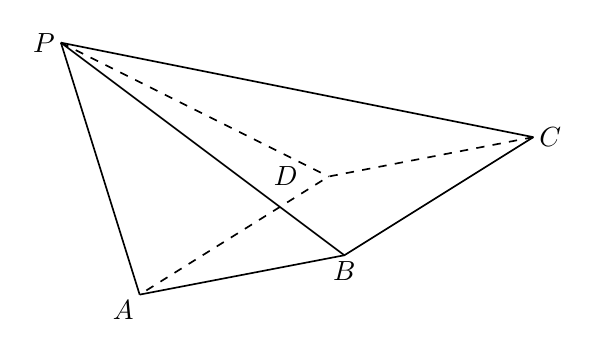
\begin{tikzpicture}[x=1cm,y=1cm,font=\normalsize,
  solidedge/.style={solid,line width=.6pt,draw=black},
  hidedge/.style={dashed,line width=.6pt,draw=black},
  ptlabel/.style={font=\normalsize,inner sep=2pt}]
\coordinate (P) at (0,3.2);
\coordinate (A) at (1,0);
\coordinate (B) at (3.6,0.5);
\coordinate (C) at (6,2);
\coordinate (D) at (3.4000000000,1.5000000000);
% 底面：可见 A-B、B-C；遮挡 C-D、D-A
\draw[solidedge] (A) -- (B) -- (C);
\draw[hidedge] (C) -- (D) -- (A);
% 底面对角线 D-B 可见
\draw[solidedge] (P)--(B);
% 侧棱：可见 P-A、P-B、P-C；遮挡 P-D
\draw[solidedge] (P) -- (A);
\draw[solidedge] (P) -- (C);
\draw[hidedge] (P) -- (D);
\node[ptlabel,left] at (P) {$P$};
\node[ptlabel,below left] at (A) {$A$};
\node[ptlabel,below] at (B) {$B$};
\node[ptlabel,right] at (C) {$C$};
\node[ptlabel,left,xshift=-9pt,yshift=0pt] at (D) {$D$};
\end{tikzpicture}
